\documentclass[conference]{IEEEtran}
\usepackage{amsmath,amsfonts}
\usepackage{algorithmic}
\usepackage{algorithm}
\usepackage{array}
\usepackage[caption=false,font=normalsize,labelfont=sf,textfont=sf]{subfig}
\usepackage{textcomp}
\usepackage{stfloats}
\usepackage{url}
\usepackage{verbatim}
\usepackage{graphicx}
\usepackage{booktabs,threeparttable}
\hyphenation{op-tical net-works semi-conduc-tor IEEE-Xplore}
% updated with editorial comments 8/9/2021
\usepackage{biblatex}
\addbibresource{references.bib}

\begin{document}

\title{Assignment template using IEEEtran.cls\\ for IEEE Journals and Transactions}

\author{
	\IEEEauthorblockN{FirstName LastName}
	\IEEEauthorblockA{
		\textit{Department of Computer Science } \\
		\textit{UiT The Arctic University of Norway}\\
		Tromsø, Norway \\
		aabbb1234@uit.no
	}
	\and
	\IEEEauthorblockN{FirstName LastName}
	\IEEEauthorblockA{
		\textit{Department of Computer Science } \\
		\textit{UiT The Arctic University of Norway}\\
		Tromsø, Norway \\
		aabbb1234@uit.no \\
		userName@github
	}
	\and
	\IEEEauthorblockN{FirstName LastName}
	\IEEEauthorblockA{
		\textit{Department of Computer Science } \\
		\textit{UiT The Arctic University of Norway}\\
		Tromsø, Norway \\
		aabbb1234@uit.no \\
		userName@github
	}
}
%\author{FirstName MiddleName(s) LastName, abc@uit.no, git username
% <-this % stops a space
%\thanks{This paper was produced by the IEEE Publication Technology Group.}}% <-this % stops a space
%\thanks{Manuscript received April 19, 2021; revised August 16, 2021.}}

% The paper headers
%\markboth{Journal of \LaTeX\ Class Files,~Vol.~14, No.~8, August~2021}%
\markboth{INF-xxxx Assignment X \today}%
{Shell \MakeLowercase{\textit{et al.}}: A Sample Article Using IEEEtran.cls for IEEE Journals}


\maketitle

\begin{abstract}
	This document describes the most common article elements and how to use the IEEEtran class with \LaTeX \ to produce files suitable for submission to the IEEE.  IEEEtran can produce conference, journal, and technical note (correspondence) papers with suitable class options.
	This template is meant as a general guideline on how to write a report, and to give some tips about what you should and should not be writing. You may move or cut sections depending on the assignment or your needs.

	While writing this report template, I enjoyed reading Michael Alley's `The Craft of Scientific Writing'. I recommend having it by your side when you are stuck writing- it happens to all of us \cite{AlleyMichael2018TCoS}.

	\bigskip

	Make sure you clean up the template text before submitting your report. ;)
\end{abstract}

\begin{IEEEkeywords}
	Assignment submission, \LaTeX, paper, template, typesetting.
\end{IEEEkeywords}

\section{Introduction}
\label{Section:Introduction}
This section should be brief. Describe the assignment and the requirements in your own words. Avoid listing the requirements directly.

\bigskip

There are many opinions on first person speaking when writing a technical report. In general:

\begin{itemize}
	\item 1. First-person report is good at:
	      \begin{itemize}
		      \item Expressing individual work, personal opinions and ideas.
		      \item Creates an informal and personal tone.
		      \item Reduces cluttering of your writing
	      \end{itemize}
	\item 2. An objective report is good at:
	      \begin{itemize}
		      \item Emphasizing your work
	      \end{itemize}
\end{itemize}


Mixing these in your reports is not uncommon, and people like Einstein, Feynman, and Curie frequently used both forms in their texts.

\bigskip

Here are some examples of how to start your introduction:

\begin{enumerate}
	\item This report describes the design and implementation of a list ADT using a linked list. It will go into detail about the design choices made and discuss the benefits and trade offs of those choices.
	\item Boids is a computer model created by Craig Reynolds that simulates the flocking behavior of birds \cite{TanenbaumAndrewS.2024Mos}. In this report, we present an implementation of the model using the Python programming language.
	\item SQL is a widely used querying language used to process queries into table-based databases. This text details the implementation of a simplified server that implements a subset of the SQL language built over sqlite.
\end{enumerate}

\subsection{Outline}
\label{Subsection:Outline}
The rest of this paper is organized as follows:


\textbf{Section~\ref{Section:Theoretical Background}} outlines concepts and background information relevant to the rest of the paper.

\textbf{Section~\ref{Section:Design}} is a high-level description of your solution to the assignment.

\textbf{Section~\ref{Section:Implementation}} goes into a detailed explanation of your implementation that you described in Section~\ref{Section:Design}.

\textbf{Section~\ref{Section:Experiments and Results}} discusses the methodology for your experiments and includes results from your experiments.

\textbf{Section~\ref{Section:Discussion}} is the most important section in a report; this is where you show that you understand the theory behind your solution and can reflect on it with the choices you made.

\textbf{Section~\ref{Section:Conclusion}} concludes and summarizing possible future work.


\section{Theoretical Background}
\label{Section:Theoretical Background}
This section is where you provide information on the theoretical aspects of your design.
You can usually assume that the theory required to solve the assignment is known to the reader, but if you want to clarify terms or go into detail about specific points in the theory (if you are doing something slightly different, or a detail of it is of notable importance to your implementation), consider writing a few words about it here.

\bigskip

We want you to write a short section explaining the most important background information required to read and understand the rest of the report.

\bigskip

Here is an example of a subsection covering a topic.

\subsection{Virtual memory}
\label{Subsection:Virtual_memory}
The basic concept of virtual memory is that you map the virtual address the processes use to a unique
physical address in physical memory. This means that two processes can access the same virtual address
in their address space but get two different results since the addresses point to different
places in the physical memory. This again means that each process can use all of its 32-bit
address space while still ensuring that no other processes can access its data~\cite{TanenbaumAndrewS.2024Mos}

\bigskip

Using figures in technical backgrounds is encouraged, if that makes the concept easier to explain. Usually, you want figures/images as Scaleable Vector Graphics(SVG) or Portable Document Format(PDF), especially for your graphs. Sometimes that is not doable, and you can use portable network graphics(PNG) or similar.
The following snippet shows how to import figures.

\begin{figure}[htbp]
	\centering
	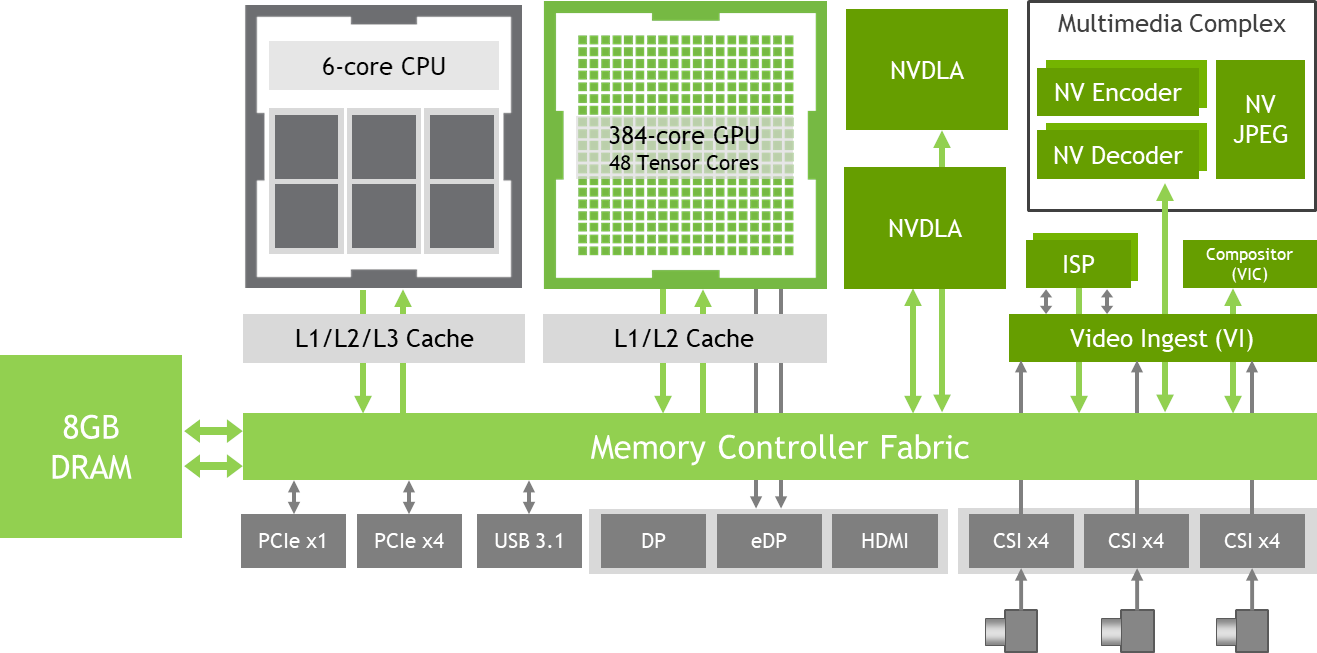
\includegraphics[scale=0.75]{figures/jetson_nx.png}
	\caption{Block diagram of the Jetson Xavier NX}
	\label{fig:block_diagram}
\end{figure}

% NOTE: Requires \usepackage{svg} and Inkscape installed
% \begin{figure}[htbp]
% 	\centering
% 	\includesvg[scale=0.5]{figures/NVSD_VDD_IN.svg}
% 	\caption{Total power consumption compared between NAS and SD-Card\newline \emph{Note} the NAS-experiment did not complete in time, and the measurements for the NAS fit to the SD-card measurements}
% 	\label{fig:local_nas_sd_compare}
% \end{figure}

\begin{figure}[htbp]
	\begin{center}
		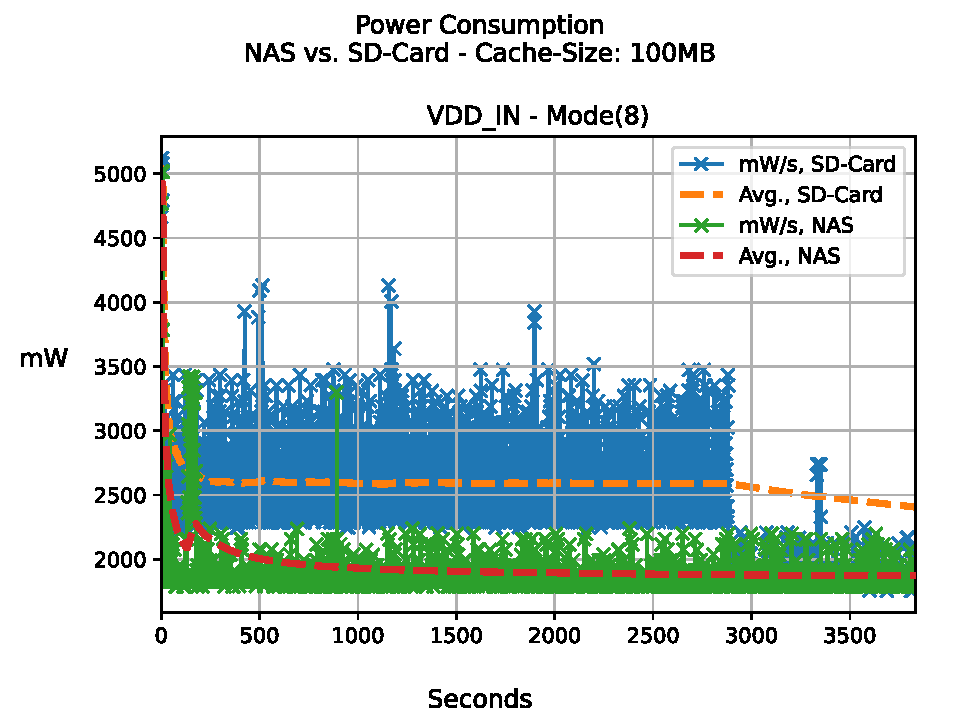
\includegraphics[width=\linewidth]{figures/NVSD_VDD_IN.pdf}
		\caption{Total power consumption compared between NAS and SD-Card\newline \emph{Note} the NAS-experiment did not complete in time, and the measurements for the NAS fit to the SD-card measurements}
		\label{fig:local_nas_sd_compare_pdf}
	\end{center}
\end{figure}

\section{Design}
\label{Section:Design}
This is where you describe how you solved the assignment, at least on paper. Give a high-level view of your design.
As a rule of thumb, if you find yourself describing code, you need to go to a higher abstraction level.


\bigskip

This section is also a good place to put illustrations to enhance the text.
There are multiple tools out there to create good illustrations.
draw.io is a strong tool that can be run in a browser. There are stronger, free tools, such as Yed Graph Editor, for more advanced users.


\bigskip

While illustrations can help make your report clearer and look more polished, avoid using them to fill up space if you can convey the same information clearly using just text.


\bigskip

Examples of what the design section should cover:

\begin{itemize}
	\item The interface of the list ADT supports six methods. These are create\_list(), destroy\_list(), add\_list(), remove\_list(), iterate\_list() and sort\_list(). When a list is created, it is provided with a comparator method that is used to handle sorting{\dots}
	\item The Boids simulation consists of a set of entities called Boids, Each boid moves independently according to a set of criteria, specified in three rules. Firstly, boids avoid crashing into obstacles, including other boids. Secondly, boids attempt to maintain the same speed and heading as nearby boids. Finally, all boids attempt to move closer to each other to form a cohesive flock.
	\item The server parses incoming data requests into an SQL query and runs them on its database. The result is then processed into JSON and returned to the client.
\end{itemize}

\bigskip

Remember to avoid low-level details! An expert should in theory be able to implement your design in any programming language based on what you write in this section.

\section{Implementation}
\label{Section:Implementation}
This is where you go into detail about your specific implementation. Questions you should answer here are things such as ``How does your implementation match your design?'' and ``Are there any bugs, and do you have any ideas about what may be causing them?''. What sort of difficulties did you experience when working, and how did you overcome them? If you found a clever solution to the problem, this is also the place to write about that.

\subsection{Technical Details}
\label{Subsection:Technical_details}
You may want to include a short section giving high-level details about your implementation, such as the programming language used and other information you find relevant for your report. In most cases however, this section is unnecessary, as the assignment usually decides those details for you. Even if you have the freedom of choice, consider whether this information is really relevant to the report, which should avoid low-level implementation details most of the time.

\section{Experiments and Results}
\label{Section:Experiments and Results}
A core pillar of computer science is testing. In this section, you should include your methodology for testing your implementation. How do you know your implementation meets the requirements? What sort of performance metrics have you chosen to benchmark your solution, and how did you go about performing tests to gather those metrics?

\bigskip

You should present the results of your tests here, either using an illustration and/or a table of results. These will be valuable in the discussion section.
The following is an example for how to format a table of results in \LaTeX.

\begin{table}[!ht]
	\begin{tabular*}{\linewidth}{@{\extracolsep{\fill}} l cc cc cc @{}}
		\toprule & \multicolumn{6}{c}{Precision} \\
		\cmidrule{2-7}
		Classifier          & (1)\tnote{a} & (2)\tnote{b}  & (3)\tnote{c}  & (1\&2)\tnote{d} & (1\&3)\tnote{e} & All\\
		\midrule
		Perceptron          & 0.78 & 0.82 & 0.24 & 0.81 & 0.77  & 0.83\\
		Decision Tree       & 0.65 & 0.79 & 0.56 & 0.75 & 0.65  & 0.73\\
		One-Class~SVM       & 0.74 & 0.72 & 0.50 & 0.80 & 0.73  & 0.85\\
		Isolation Forest    & 0.54 & 0.51 & 0.52 & 0.53 & 0.54  & 0.53\\
		\bottomrule
		\newline
	\end{tabular*}
	\caption{Precision results of classifiers for different feature sets}
	\label{table:testing}
\end{table}


\bigskip

If presenting data and benchmarks are not important to the assignment, you may likely find yourself cutting this section. If you decide to do so, make sure you at least mention your correctness criteria and testing methodology somewhere else.

\section{Discussion}
\label{Section:Discussion}
The discussion section is the most important section in a report, This is where you show that you understand the theory behind the solution, and also a chance to argue the pros and cons of your solution. You should discuss about the results of your measurements and why you think they are the way they are. Also bring up tradeoffs, and why you made the choices you did; show that you understand the alternatives, and why they may be a good idea (or not) for the particular problem the assignment asked you to solve.

\bigskip

Here is an example of a discussion subsection:

\subsection{Recovery of a simulated crash}
\label{Subsection:Recovery_simulated_crash}
When a node recovers from a simulated crash, it will check if it's neighbors is still connected to it. If not, it will try and start an internal join to its previous successor. This works as long as the previous successor is still active in the network. The case where the previous successor is not active, is not dealt with, and will result in the node not being able to recover.


\section{Conclusion}
\label{Section:Conclusion}
Here you sum up the report and reiterate the results. Does not need to be very long, a few sentences is fine.


\printbibliography

{\appendix[Proof of the Zonklar Equations]
	Use $\backslash${\tt{appendix}} if you have a single appendix:
	Do not use $\backslash${\tt{section}} anymore after $\backslash${\tt{appendix}}, only $\backslash${\tt{section*}}.
	If you have multiple appendixes use $\backslash${\tt{appendices}} then use $\backslash${\tt{section}} to start each appendix.
	You must declare a $\backslash${\tt{section}} before using any $\backslash${\tt{subsection}} or using $\backslash${\tt{label}} ($\backslash${\tt{appendices}} by itself
	starts a section numbered zero.)}

%{\appendices
%\section*{Proof of the First Zonklar Equation}
%Appendix one text goes here.
% You can choose not to have a title for an appendix if you want by leaving the argument blank
%\section*{Proof of the Second Zonklar Equation}
%Appendix two text goes here.}


\end{document}
